\documentclass[11pt]{article}

\usepackage{float}
\usepackage{hyperref}
\usepackage{graphicx}
% formatting
\usepackage{verbatim}
\usepackage{moreverb}
\usepackage{minted}
\usepackage{parskip}
\usepackage{amsmath}
\usepackage[listings]{tcolorbox}
\usepackage{enumerate}
\usepackage{tikz}
\usetikzlibrary{arrows,automata, positioning}
\let\verbatiminput=\verbatimtabinput
\def\verbatimtabsize{4\relax}

\newcommand{\RepoRootPath}{fpga\_labs\_fa19}

\tcbset{
texexp/.style={colframe=black, colback=lightgray!15,
         coltitle=white,
         fonttitle=\small\sffamily\bfseries, fontupper=\small, fontlower=\small},
     example/.style 2 args={texexp,
title={Question \thetcbcounter: #1},label={#2}},
}

\newtcolorbox{texexp}[1]{texexp}
\newtcolorbox[auto counter]{texexptitled}[3][]{%
example={#2}{#3},#1}

\setlength{\topmargin}{-0.5in}
\setlength{\textheight}{9in}
\setlength{\oddsidemargin}{0in}
\setlength{\evensidemargin}{0in}
\setlength{\textwidth}{6.5in}

% Useful macros

\newcommand{\note}[1]{{\bf [ NOTE: #1 ]}}
\newcommand{\fixme}[1]{{\bf [ FIXME: #1 ]}}
\newcommand{\wunits}[2]{\mbox{#1\,#2}}
\newcommand{\um}{\mbox{$\mu$m}}
\newcommand{\xum}[1]{\wunits{#1}{\um}}
\newcommand{\by}[2]{\mbox{#1$\times$#2}}
\newcommand{\byby}[3]{\mbox{#1$\times$#2$\times$#3}}


\newenvironment{tightlist}
{\begin{itemize}
 \setlength{\parsep}{0pt}
 \setlength{\itemsep}{-2pt}}
{\end{itemize}}

\newenvironment{titledtightlist}[1]
{\noindent
 ~~\textbf{#1}
 \begin{itemize}
 \setlength{\parsep}{0pt}
 \setlength{\itemsep}{-2pt}}
{\end{itemize}}

% Change spacing before and after section headers

\makeatletter
\renewcommand{\section}
{\@startsection {section}{1}{0pt}
 {-2ex}
 {1ex}
 {\bfseries\Large}}
\makeatother

\makeatletter
\renewcommand{\subsection}
{\@startsection {subsection}{1}{0pt}
 {-1ex}
 {0.5ex}
 {\bfseries\normalsize}}
\makeatother

% Reduce likelihood of a single line at the top/bottom of page
\clubpenalty=2000
\widowpenalty=2000

% Other commands and parameters
\pagestyle{myheadings}
\setlength{\parindent}{0in}
\setlength{\parskip}{10pt}

% Commands for register format figures.
\newcommand{\instbit}[1]{\mbox{\scriptsize #1}}
\newcommand{\instbitrange}[2]{\instbit{#1} \hfill \instbit{#2}}

% Break lines on texttt text on underscores
% See: https://tex.stackexchange.com/questions/315369/how-to-deal-with-bad-line-wrapping-of-texttt
\newcommand*\ttvar[1]{\texttt{\expandafter\dottvar\detokenize{#1}\relax}}
\newcommand*\dottvar[1]{\ifx\relax#1\else
  \expandafter\ifx\string_#1\string_\allowbreak\else#1\fi
  \expandafter\dottvar\fi}

\begin{document}

\def\PYZsq{\textquotesingle}
\title{\vspace{-0.4in}\Large \bf EECS 151/251A FPGA Lab 5:\\FSMs and UART \vspace{-0.1in}}

\author{Prof. Borivoje Nikolic and Prof. Sophia Shao \\
TAs: Cem Yalcin, Rebekah Zhao, Ryan Kaveh, Vighnesh Iyer \\ Department of Electrical Engineering and Computer Sciences\\
College of Engineering, University of California, Berkeley}
\date{}
\maketitle

\newcommand{\headertext}{EECS 151/251A FPGA Lab 5: FSMs and UART}
\markboth{\headertext}{\headertext}
\thispagestyle{empty}

\section{Music Streamer FSM}
Implement a simple FSM in the \verb|music_streamer|.

The FSM has 3 states: \verb|PAUSED|, \verb|REGULAR_PLAY|, \verb|REVERSE_PLAY|.
Here is the state transition diagram:
\begin{center}
\begin{tikzpicture}[shorten >=1pt, node distance=10cm,on grid, auto,line width=0.05cm]
  \tikzstyle{state} = [draw, very thick, fill=white, rectangle, minimum height=3em, minimum width=7em, node distance=17em, font={\sffamily\bfseries}]
  \tikzstyle{stateEdgePortion} = [black,thick];
  \tikzstyle{stateEdge} = [stateEdgePortion,->,line width=3cm];
  \tikzstyle{edgeLabel} = [pos=0.5, text centered, font={\sffamily\small}];

  \node[state,initial](rp) {REGULAR\_PLAY};
  \node[state](revp) [below =of rp]{REVERSE\_PLAY};
  \node[state](p) [right=of rp]{PAUSED};

  \path[->]
  (rp) edge node {Play-pause button} (p)
    edge [swap] node {Reverse button} (revp)
    edge [loop above] node {} (rp)
  (p) edge node {} (rp)
    edge [loop below] node {} (p)
  (revp) edge [swap] node {Play-pause button} (p)
    edge [swap] node {} (rp)
    edge [loop below] node {} (revp);
\end{tikzpicture}
\end{center}

\begin{enumerate}
  \item The initial state should be \verb|REGULAR_PLAY|.
  \item Pressing the \verb|play_pause| button should transition you into the \verb|PAUSED| state from either the \verb|REGULAR_PLAY| or \verb|REVERSE_PLAY| states. Pressing the same button while in the \verb|PAUSED| state should transition the FSM to the \verb|REGULAR_PLAY| state.
  \item In the \verb|PAUSED| state, the ROM address should be held steady at its value before the transition into \verb|PAUSED| and no sound should come out of the speaker. After leaving the \verb|PAUSED| state the ROM address should begin incrementing again from where it left off and the speaker should play the tones.
  \item You can toggle between the \verb|REGULAR_PLAY| and \verb|REVERSE_PLAY| states by using the \verb|reverse| button. In the \verb|REVERSE_PLAY| state you should decrement the ROM address by 1 rather than incrementing it by 1 every X clock cycles as defined by the tempo.
  \item If you don't press any buttons, the FSM shouldn't transition to another state.
\end{enumerate}

The \verb|music_streamer| takes in user button inputs (\verb|play_pause, reverse|) that it can use to transition states.

Also, drive the LEDs such that they show the current state. An example:
\renewcommand{\arraystretch}{1.5}
\begin{center}
\begin{tabular}{| l | l |}
  \hline
  \textbf{LED} & \textbf{Value} \\ \hline
      leds[0] & \verb|current_state| == \verb|REGULAR_PLAY| \\ \hline
      leds[1] & \verb|current_state| == \verb|PAUSED| \\ \hline
      leds[2] & \verb|current_state| == \verb|REVERSE_PLAY| \\ \hline
\end{tabular}
\end{center}

Look at the commented code in \ttvar{music_streamer_testbench.v} that tests the state machine.
Uncomment and run the test and inspect the waveform to check that the FSM is performing correctly.

Next, modify \verb|z1top.v| to connect the \verb|play_pause| and \verb|reverse| ports to \verb|buttons_pressed| [2] and [3] respectively.

Finally, program the FPGA with the \verb|music_streamer|, and verify its functionality.

\section{Checkoff}
\begin{enumerate}
  \item Show the RTL for the input conditioning circuits and music streamer
  \item Play an audio file generated from a simulation
  \item Demonstrate the music streamer on the FPGA (FSM, tempo control, reset)
\end{enumerate}

\subsection{Lab Report}
Submit a short report containing the waveform screenshots to answer the questions in the lab.

\section*{Ackowlegement}
This lab is the result of the work of many EECS151/251 GSIs over the years including:
\begin{itemize}
\item Sp12: James Parker, Daiwei Li, Shaoyi Cheng
\item Sp13: Shaoyi Cheng, Vincent Lee
\item Fa14: Simon Scott, Ian Juch
\item Fa15: James Martin
\item Fa16: Vighnesh Iyer
\item Fa17: George Alexandrov, Vighnesh Iyer, Nathan Narevsky
\item Sp18: Arya Reais-Parsi, Taehwan Kim
\item Fa18: Ali Moin, George Alexandrov, Andy Zhou
\end{itemize}

\end{document}
